\section{Rekonstruktion toteutus}
Säteen lävistämien kuva-alueen vokseleiden laskentaan Siddonin algoritmilla tarvitaan kaksi pistettä säteen virittämältä suoralta avaruudessa kuva-alueen parametrien lisäksi\cite{sundermann_fast_1998}. Koska epäideaalin kollimaattorin reikä kerää säteilyä kartion muotoiselta alueelta avaruudessa, jokaiselle detektorin pikselille asetetaan useampi säde kollimaattorin reikien sisälle. Kunkin säteen lävistämät vokselit ja pituudet niissä määritetään, jonka jälkeen pituudet keskiarvoistetaan vokselikohtaisesti. Projektion lasketaan käytetään näitä keskiarvoja.

\subsection{Kollimaattorin mallinnus}
Työssä toteutettiin kaksi eri mallia kollimaattorille, jonka reiät ovat suoria särmiöitä kuusikulmaisella pohjalla. Toinen malli on kehitetty mahdollisimman todenmukaista rekonstruktiota varten ja toinen laskentatehokkuutta ajatellen.

Kummassakin mallissa kollimaattorin yksittäisen reiän ajatellaan koostuvan sisäkkäisistä kuusikulmaisista suorista särmiöistä. Jokaiselle särmiölle muodostetaan kuusi avaruuslävistäjää, jotka toimivat projektion laskennassa tarvittavina säteinä. Ennen laskentaa kuitenkin tarkistetaan vielä, että säteet osuvat oikeaan pikseliin detektorissa. \hyperref[fig:ray1]{Kuva \ref*{fig:ray1}} havainnollistaa detektoripaneelin tasoa ja kollimaattorin malleja. Tasolle on rajattu detektorin pikselit punaisella viivalla ja säteiden päätepisteet sinisillä pisteillä.

\begin{figure}[t]
    \centering
    \captionsetup{width=.9\textwidth}
    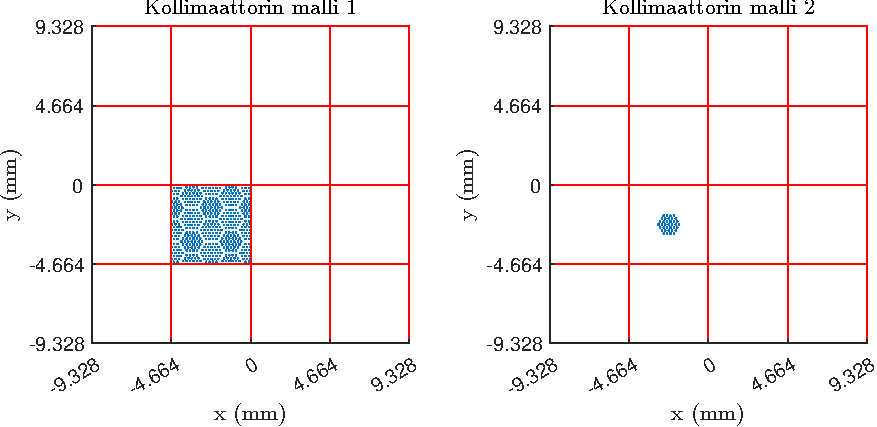
\includegraphics[width=.9\textwidth]{kuvat/2d-kollimaattori.pdf}
    \caption{Detektoripaneelin taso. Detektorin pikselit ovat rajattu punaisilla viivoilla ja kollimaattorin reikien sisälle yhden pikselin alueella on asetettu tasaisesti pisteitä sinisellä värillä. Vasemmalla puolella, mallissa 1, säteitä on 543 ja oikealla puolella, mallissa 2, säteitä on 37. Kollimaattorin reiän halkaisija on \qty{1.4}{\milli\meter} ja reikien väli on \qty{0.12}{\milli\meter}. Detektorin pikselin koko on \qty{4.664}{\milli\meter}.}
    \label{fig:ray1}
\end{figure}

Ensimmäisessä mallissa kollimaattorin reiät ovat todenmukaisissa paikoissaan. \hyperref[fig:ray1]{Kuvan \ref*{fig:ray1}} vasemmassa laidassa esitetty malli sisältää 543 sädettä, kun yhdessä kollimaattorin reiässä on 37 sädettä. \hyperref[fig:ray1]{Kuvan \ref*{fig:ray1}} oikeassa laidassa esitetty toinen malli muodostuu vain yhdestä kollimaattorin reiästä detektorin pikseliä kohti. 

Kuviin \ref{fig:ray2} ja \ref{fig:ray3} on piirretty kuva-alue kolmiulotteisessa avaruudessa mustalla ruudukolla ja detektorin yhdelle pikselille asettuvat säteet sinisillä viivoilla. \hyperref[fig:ray2]{Kuvassa \ref*{fig:ray2}} on käytetty todenmukaisempaa mallia 98 säteellä, jolloin jokaista kollimaattorin reikää kohti jää 7 sädettä. Seitsemän säteen kuvio on selvästi nähtävissä suuremmassakin mittakaavassa.

\begin{figure}[H]
    \centering
    \captionsetup{width=.9\textwidth}
    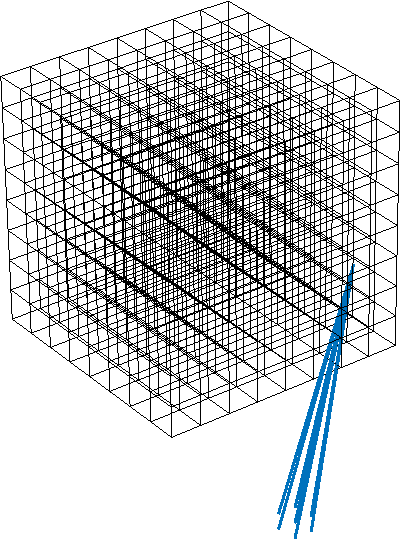
\includegraphics[height=6cm]{kuvat/3d-kollimaattori1.pdf}
    \caption{Kollimaattorin mallin 1 havainnollistus kolmiulotteisessa avaruudessa. Kuva-alue on piirretty mustalla ruudukolla ja detektorin havaitsemat säteet (98 kappaletta) sinisellä värillä. Kollimaattorin reiän pituus on \qty{32.4}{\milli\meter}, reiän halkaisija on \qty{1.4}{\milli\meter} ja reikien välinen etäisyys on \qty{0.12}{\milli\meter}. Detektorin pikselin koko on \qty{4.664}{\milli\meter}. Yksi ruudukon kuutio vastaa $8^3$ vokselia, jossa yksittäisen vokselin koko on $(\qty{4.664}{\milli\meter})^{3}$.}
    \label{fig:ray2}
\end{figure}

\hyperref[fig:ray3]{Kuvassa \ref*{fig:ray3}} on esitetty jälleen kuva-alue mustalla ruudukolla ja detektorin yhdelle pikselille asettuvat säteet sinisillä viivoilla. Kuvaan on piirretty yhteensä 61 sädettä mallilla 2. Kuvista nähdään, kuinka detektorin havaitsema alue avaruudesta täyttyy tasaisemmin yhden reiän mallilla, vaikka säteitä on yli kolmannes vähemmän.

\begin{figure}[H]
    \centering
    \captionsetup{width=.9\textwidth}
    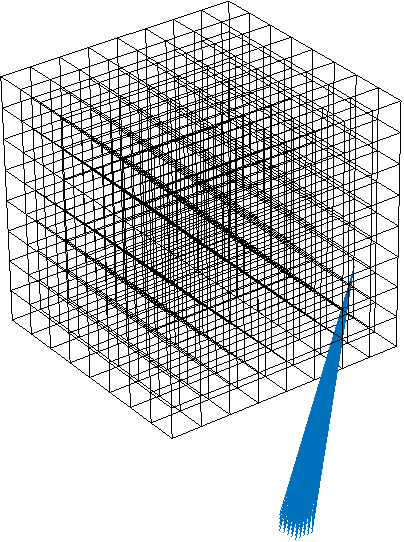
\includegraphics[height=6cm]{kuvat/3d-kollimaattori2.pdf}
    \caption{Kollimaattorin mallin 2 havainnollistus kolmiulotteisessa avaruudessa. Kuva-alue on piirretty mustalla ruudukolla ja detektorin havaitsemat säteet (61 kappaletta) sinisellä värillä. Kollimaattorin reiän pituus on \qty{32.4}{\milli\meter}, reiän halkaisija on \qty{1.4}{\milli\meter} ja reikien välinen etäisyys on \qty{0.12}{\milli\meter}. Detektorin pikselin koko on \qty{4.664}{\milli\meter}. Yksi ruudukon kuutio vastaa $8^3$ vokselia, jossa yksittäisen vokselin koko on $(\qty{4.664}{\milli\meter})^{3}$.}
    \label{fig:ray3}
\end{figure}

\subsection{Koodin toiminta}
Kollimaattorin mallintava koodi kehitettiin MATLAB-ympäristössä \textcolor{red}{(R2023b, Mathworks Inc.)} testauksen nopeuden ja helppouden vuoksi. Toimivassa versiossa hyödynnettiin eräitä MATLABin funktioita, joita ei ole C++:n vakiokirjastossa. Näitä ovat muun muuassa trigonometriset funktiot, joiden argumenttina on kulma asteina sekä \texttt{floorDiv}, joka laskee ensin kahden luvun osamäärän ja pyöristää sen alaspäin lähimpään kokonaislukuun. Koodin luettavuuden kannalta on helpompaa toteuttaa nämä erillisinä apufunktioina C++:ssa. Apufunktiot kokonaisuudessaan ovat esitetty \hyperref[appendix:apufunktiot]{liitteessä \ref*{appendix:apufunktiot}}.

\textcolor{red}{2D siirto \hyperref[appendix:2Dsiirto]{Liite \ref*{appendix:2Dsiirto}}}

Parametreinä kummassakin mallissa ovat detektorin pikselin koko, pikselin indeksi detektoripaneelissa, kollimaattorin reiän halkaisija, reiän pituus, reikien välinen etäisyys (\textit{septal width}), kuusikulmaisen reiän suuntaus ja säteiden lukumäärä. Reiän suuntauksessa arvo 1 asettaa kuusikulmion kärjet detektoripaneelin tason $x$-akselin suuntaisesti ja arvo 2 $y$-akselin suuntaisesti.

Pääfunktion \texttt{computeSpectHexShifts} parametrit ovat esitetty myös \hyperref[tbl:parametrit]{Taulukossa \ref*{tbl:parametrit}}.
\begin{table}[H]
    \centering
    \captionsetup{width=.9\textwidth}
    \caption{Funktion \texttt{computeSpectHexShifts} parametrit}
    \resizebox{.9\textwidth}{!}{%
        \begin{tabular}{lcc}
            \toprule
            Parametrin nimi & Arvo & Kuvaus \\
            \midrule
            \texttt{param.coneMethod} & $\left\{ 1, 2 \right\}$ & Mallin valinta \\
            \texttt{param.hexOrientation} & $\left\{ 1, 2 \right\}$ & Kuusikulmion pohjan suuntaus \\
            \texttt{param.nRaySPECT} & $\mathbb{N}$ & Säteiden lukumäärä yhdessä kollimaattorin reiässä \\
            \texttt{param.dPitchXY} & $>0$ & Detektorin pikselin reunan pituus \\
            \texttt{param.colL} & $>0$ & Kollimaattorin reiän pituus \\
            \texttt{param.colD} & $>0$ & Kollimaattorin reiän halkaisija \\
            \texttt{param.dSeptal} & $>0$ & Kollimaattorin reikien välinen etäisyys \\
            \texttt{detectors.xd} & $\mathbb{R}$ & Detektorin pikselin keskipisteen $x$-koordinaatti \\
            \texttt{detectors.yd} & $\mathbb{R}$ & Detektorin pikselin keskipisteen $y$-koordinaatti \\
            \texttt{detectors.zd} & $\mathbb{R}$ & Detektorin pikselin keskipisteen $z$-koordinaatti \\
            \texttt{detectors.xs} & $\mathbb{R}$ & \texttt{detectors.xd} + detektoripaneelin sisänormaalivektorin $x$-komponentti \\
            \texttt{detectors.ys} & $\mathbb{R}$ & \texttt{detectors.yd} + detektoripaneelin sisänormaalivektorin $y$-komponentti \\
            \texttt{detectors.zs} & $\mathbb{R}$ & \texttt{detectors.zd} + detektoripaneelin sisänormaalivektorin $z$-komponentti \\
            \texttt{ix} & $\mathbb{N}$ & Detektorin pikselin indeksi paneelin $x$-suunnassa \\
            \texttt{iy} & $\mathbb{N}$ & Detektorin pikselin indeksi paneelin $y$-suunnassa \\
            \bottomrule
        \end{tabular}
    }
    \label{tbl:parametrit}
\end{table}

\textcolor{red}{3D siirto \hyperref[appendix:3Dsiirto]{Liite \ref*{appendix:3Dsiirto}}}

\subsection{Integraatio OMEGAan}
\textcolor{red}{Aiempien koodien muokkaukset (projector\_mex, projector\_functions, SPECT\_mainMOD), sinogrammin muuntaminen \texttt{x}-muuttujaan, GitHub, yms.}